

\documentclass{acm_proc_article-sp}


\usepackage{graphicx}
\usepackage{listing}
\usepackage{listings} \lstset{basicstyle=\tiny,numbers=none, breaklines=true, numberstyle=\tiny, numbersep=5pt,firstnumber=last,language=XML,escapeinside={(*@}{@*)} }  

% *** CITATION PACKAGES ***
%
\usepackage{cite}
\usepackage{url}
%\usepackage[scaled=point85]{luximono}
\hyphenation{op-tical net-works semi-conduc-tor name-space}

\begin{document}

\title{VIENNA Add-In \\ Visualizing Inter-ENterprise Network Architectures}


%Do not change this number
\numberofauthors{2}


\author{
% You can go ahead and credit any number of authors here,
% e.g. one 'row of three' or two rows (consisting of one row of three
% and a second row of one, two or three).
%
% The command \alignauthor (no curly braces needed) should
% precede each author name, affiliation/snail-mail address and
% e-mail address. Additionally, tag each line of
% affiliation/address with \affaddr, and tag the
% e-mail address with \email.
%
% 1st. author
\alignauthor
Christian Huemer, Philipp Liegl, Thomas Motal, Rainer Schuster, Marco Zapletal \\
       \affaddr{Vienna University of Technology}\\
       \affaddr{Favoritenstrasse 9-11/188}\\
       \affaddr{1040 Vienna, Austria}\\
       \email{\{firstname.lastname\}@tuwien.ac.at}       
\alignauthor
Christian Eis, Martina Hiesinger, Fabian Kromer, Robert Kromer, Andreas Kuntner, Christian Pichler, Michael Strommer\\
       \affaddr{Research Studios Austria}\\
       \affaddr{Thurngasse 8/3/20}\\
       \affaddr{1090 Vienna, Austria}\\
       \email{office.ios@researchstudio.at}       
% 2nd. author
%\alignauthor
%Christian Pichler\\
%       \affaddr{Research Studios Austria}\\
%       \affaddr{Thurngasse 8/3/20}\\
%       \affaddr{1090 Vienna, Austria}\\
%       \email{cpichler@researchstudio.at}
}

\date{28 April 2009}

\maketitle
\begin{abstract}

%What is the problem
The definition of concise and interoperable business documents has become one of the key issues in today's electronic business transactions. 
In this paper, we present our tool VIENNA Add-In which supports a business document modeler in creating Core Component compliant business document models using the Unified Modeling Language (UML). The core components standard is maintained by UN/CEFACT (United Nations Center for Trade Facilitation and Electronic Business) and defines reusable building blocks for constructing business documents. 
Our tool provides a set of powerful features for core components such as model validation, semi-automatic generation of model artifacts, and generation of fully compliant XML schema definitions from a conceptual model representation. Thereby, the VIENNA Add-In helps to shorten development cycles and helps to reduce errors in designing business documents. The overall goal of our tool-based approach for inter-organizational processes is the generation of deployment artifacts for IT systems from conceptual models.


\end{abstract}

% A category with the (minimum) three required fields
\category{H.4}{Information Systems Applications}{Miscellaneous}


\terms{Business document modeling, conceptual modeling, XML schema generation}


\section{Introduction}

Before two business partners can engage in an automated B2B interaction two agreements have to be made. First, the process choreography has to be specified i.e. the exact exchange order of the different business documents. Second, the business information being exchanged in the electronic transaction must be specified i.e. the business document definition. In a joint effort between the Vienna University of Technology and the Research Studios Austria, Studio Inter-Organisational Systems we have developed the VIENNA Add-In \cite{man:VIENNAAddIn}. The VIENNA Add-In support both, business choreography definitions and business document definitions. For the former the supported technology is UN/CEFACT's Modeling Methodology (UMM) \cite{man:umm2} and for the latter the UML Profile for UN/CEFACT's Core Components (UPCC) \cite{man:upcc}. Our tool demonstration will in particular focus on the business documents specific features. 

Figure \ref{fig:viennaaddinoverview} gives a brief overview of the main approach pursued by the VIENNA Add-In. 
\begin{figure}
 \centering
   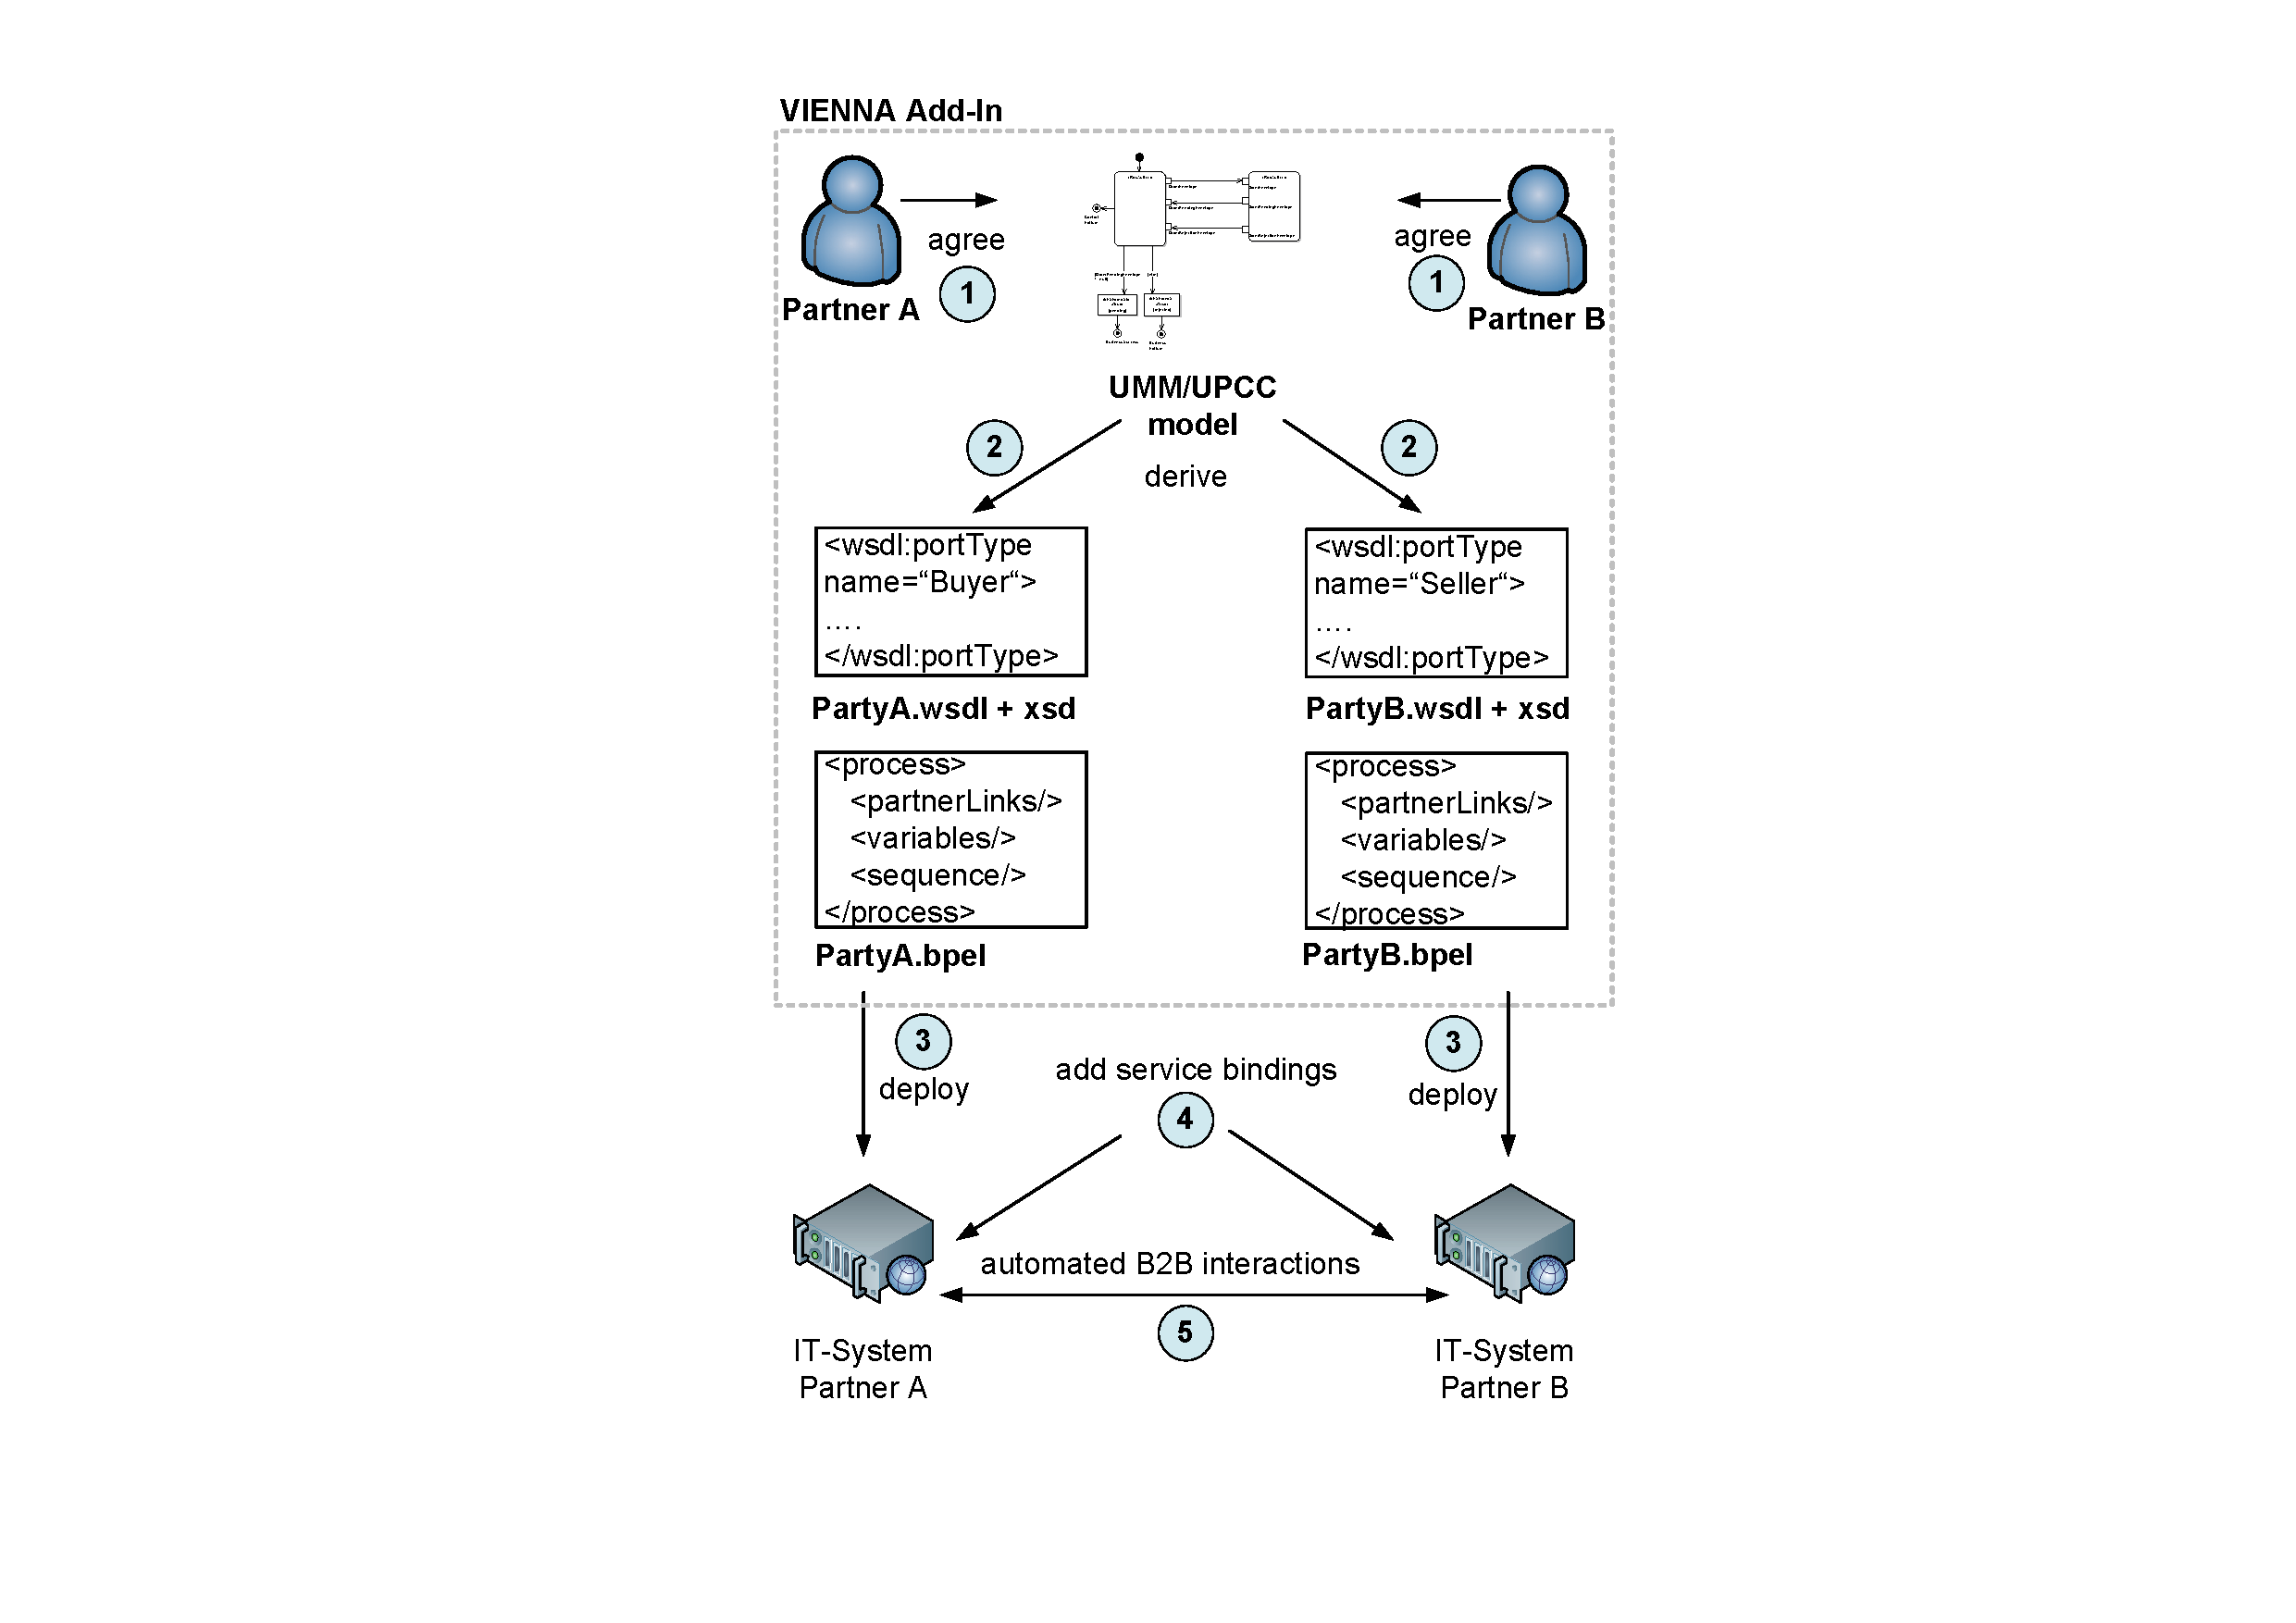
\includegraphics[width=0.32\textwidth]{figures/addinoverview.pdf}
 \caption{VIENNA Add-In overview}
 \label{fig:viennaaddinoverview}
\end{figure}
Two business partners willing to engage in an electronic collaboration first agree on a common UMM model specifying the business choreography and a common UPCC model specifying the exchanged business information ((1) in Figure \ref{fig:viennaaddinoverview}). Both models are specified on a conceptual level using the Unified Modeling Language (UML). In a consecutive step the commonly agreed upon process and information model is used to derive deployment artifacts for the IT systems (2). Interface definitions and the exchanged information is reflected using WSDL and XML Schema artifacts. The local choreography definitions are reflected using BPEL artifacts. Eventually the generated artifacts can be deployed to Business Service Interfaces (3). After adding service bindings (4) automatic B2B interactions are feasible (5). Thus, the business modeler is provided with a model driven approach for the definition of deployment artifacts for a service oriented systems.


\section{UML Profile Definition}

\section{Semi-automatic artifact generation}

\section{XML schema generation}




\bibliographystyle{abbrv}
\bibliography{references}  
\end{document}
